\documentclass[aspectratio=169]{beamer}

\mode<presentation>
\usetheme{Boadilla}
\definecolor{NTHU1}{RGB}{127,16,132}
\definecolor{NTHU2}{RGB}{228,210,231}
\definecolor{blue}{RGB}{30,90,205}
\definecolor{red}{RGB}{213,94,0}
\definecolor{green}{RGB}{0,128,0}
\definecolor{charcoalgray}{RGB}{108,104,104}
\setbeamercolor{title}{fg=NTHU1}
\setbeamercolor{frametitle}{fg=NTHU1}
\setbeamercolor{block title}{bg=NTHU1, fg=white}
\setbeamercolor{block body}{bg=NTHU2}
\setbeamercolor{structure}{fg=NTHU1}
\setbeamercolor{item projected}{fg=white}
\setbeamercolor{item}{fg=NTHU1}
\setbeamercolor{subitem}{fg=NTHU1}
\setbeamercolor{section in toc}{fg=NTHU1}
\setbeamercolor{description item}{fg=NTHU1}
\setbeamercolor{caption name}{fg=NTHU1}
\setbeamercolor{button}{bg=NTHU1, fg=white}
\setbeamercolor{caption name}{fg=NTHU1}
\usepackage{graphics}
\usepackage{tikz}
\usepackage{amsmath}
\usepackage{bbm}
\usetikzlibrary{decorations.pathreplacing}
\usepackage{geometry}
\usepackage{booktabs}
\usepackage{bookmark}
\usepackage{multirow, makecell}
\usepackage{float}
\usepackage{fancyvrb}
\usepackage{caption}
\captionsetup[figure]{singlelinecheck = false, format= hang, justification=centering}
\captionsetup[subfigure]{singlelinecheck = false, format= hang, justification=raggedright}
\usepackage{subcaption}
\usepackage{adjustbox}
\usepackage{hyperref}
\usepackage{threeparttable}
\usepackage{appendixnumberbeamer} 
\usepackage[T1]{fontenc}
\usepackage[default]{lato} 
\usepackage{smartdiagram}
\smartdiagramset{
  back arrow disabled = true,
  module minimum width=1cm,
  module x sep = 3,
  uniform arrow color=true,
}
\usepackage{xcolor}
\usepackage{colortbl}
	\definecolor{light-gray}{gray}{0.99}

\newenvironment{wideitemize}{\itemize\addtolength{\itemsep}{10pt}}{\enditemize}
\newenvironment{wideenumerate}{\enumerate\addtolength{\itemsep}{10pt}}{\endenumerate}
\newenvironment{widedescription}{\description\addtolength{\itemsep}{10pt}}{\enddescription}
\hypersetup{
colorlinks=true,
linkcolor=NTHU1,
filecolor=green, 
urlcolor=blue,
}
\beamertemplatenavigationsymbolsempty
\setbeamercolor{author in head/foot}{bg=white, fg=NTHU1}
\setbeamercolor{title in head/foot}{bg=white, fg=NTHU1}
\setbeamercolor{date in head/foot}{bg=white, fg=NTHU1}
\setbeamercolor{section in head/foot}{bg=white, fg=NTHU1}
\setbeamercolor{headline}{bg=white}
\setbeamertemplate{footline}{
    \leavevmode%
    \hbox{%
        \begin{beamercolorbox}[wd=.333333\paperwidth,ht=2.25ex,dp=1ex,center]{date in head/foot}%
            \usebeamerfont{date in head/foot}%\insertdate
        \end{beamercolorbox}%
        \begin{beamercolorbox}[wd=.333333\paperwidth,ht=2.25ex,dp=1ex,center]{title in head/foot}%
            \usebeamerfont{title in head/foot}\insertshorttitle
        \end{beamercolorbox}%
        \begin{beamercolorbox}[wd=.333333\paperwidth,ht=2.25ex,dp=1ex,right]{date in head/foot}%
            \usebeamerfont{date in head/foot}\insertframenumber{}\hspace*{2em}
        \end{beamercolorbox}}%
        \vskip0pt%
    }
    %% May need to script the introduction!!!!!!
%\setbeamercolor{page number in head/foot}{fg=NTHU1}
\setbeamertemplate{section in toc}[sections numbered]
\setbeamertemplate{subsection in toc}{\leavevmode\leftskip=3em\rlap{\hskip-1.75em\inserttocsectionnumber.\inserttocsubsectionnumber}
\inserttocsubsection\par}
\setbeamerfont{subsection in toc}{size=\footnotesize}
%\setbeamertemplate{headline}{%
  %\begin{beamercolorbox}[ht=5.5ex]{section in head/foot}
    %\vskip2pt\insertnavigation{0.33\paperwidth}\vskip2pt
  %\end{beamercolorbox}%
%}
\newenvironment{transitionframe}{\setbeamercolor{background canvas}{bg=white}\setbeamertemplate{footline}{} \begin{frame}[noframenumbering]}{\end{frame}}


\makeatletter
\let\@@magyar@captionfix\relax
\makeatother


\title[]{Public Economics and Development} % Change this regularly
\subtitle[]{Week 4: Classic Optimal Taxation Theories}
\author[Lee]{Seung-hun Lee }
\institute[]{Taipei School of Economics\\ National Tsing Hua University}

\date[]{March 17th, 2026}

\begin{document}
\begin{transitionframe}
\titlepage
\end{transitionframe}


%%% Color slides for section headers: Use for colloquium version (The ones bewteen \iffals and \fi)
\begin{transitionframe}
\frametitle{Roadmap for today}
\tableofcontents
\end{transitionframe}


\section{Basic tools of public economics}
\begin{frame}
\frametitle{Public economics as study of taxation} 
Quantifying the gains and costs of taxation
\begin{itemize}\setlength\itemsep{3pt}
\item All taxes are based on observable indicators - labor earnings, transactions  etc
\item People respond to taxes by adjusting their behaviors
\begin{itemize}\setlength\itemsep{3pt}
\item Income tax$\uparrow$ $\Rightarrow$ Opportunity cost of labor $\uparrow$  $\Rightarrow$ Labor $\downarrow$, Leisure $\uparrow$
\item Consumption tax$\uparrow$ $\Rightarrow$ Consumer price $\uparrow$ $\Rightarrow$ Transaction $\downarrow$
\end{itemize}
\item This leads to efficiency costs (deadweight loss): lower labor and lost transactions 
\begin{itemize}\setlength\itemsep{3pt}
\item Lost production and income due to less labor
\item Transactions that would have occurred pre-tax no longer exists
\end{itemize}
\item How to capture this cost, and is this cost bearable? (more on this in normative analysis)
\end{itemize}
\end{frame}


\begin{frame}
\frametitle{Graphical description of taxes in supply-demand framework}
\begin{columns}
\begin{column}{0.5\textwidth}
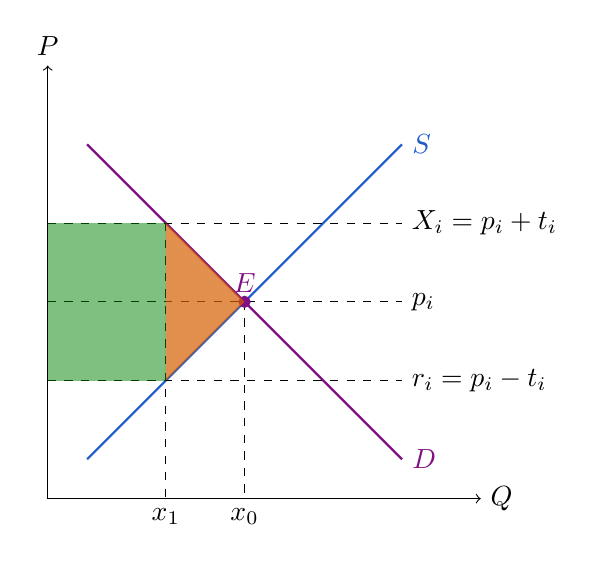
\begin{tikzpicture}[scale=1.0]
  %% 1. Axes
  \draw[->] (0,0) -- (5.5,0) node[right] {$Q$};
  \draw[->] (0,0) -- (0,5.5) node[above] {$P$};
  %% 2. Curves
  \draw[thick, color=NTHU1] (0.5,4.5) -- (4.5,0.5) node[right] {$D$};
  \draw[thick, color=blue]  (0.5,0.5) -- (4.5,4.5) node[right] {$S$};
  \draw[dashed, color=black]  (0,2.5) -- (4.5,2.5) node[right] {$p_i$};
  \draw[dashed, color=black]  (0,3.5) -- (4.5,3.5) node[right] {$X_i=p_i+t_i$};
  \draw[dashed, color=black]  (0,1.5) -- (4.5,1.5) node[right] {$r_i=p_i-t_i$};
  \draw[dashed, color=black]  (1.5,3.5) -- (1.5,0) node[below] {$x_1$};
  \draw[dashed, color=black]  (2.5,2.5) -- (2.5,0) node[below] {$x_0$};
  %% 3. Points and labels

  
  \filldraw[NTHU1] (2.5,2.5) circle (2pt) node[above] {$E$};
  %% 4. Shaded regions
  \fill[red, opacity=0.7] (1.5,1.5) -- (1.5,3.5) -- (2.5,2.5) -- cycle;
  \fill[green, opacity=0.5] (0,1.5) -- (1.5,1.5) -- (1.5,3.5) -- (0,3.5) -- cycle;
\end{tikzpicture}
\end{column}
\begin{column}{0.5\textwidth}
Pre-tax
\begin{itemize}\setlength\itemsep{3pt}
\item At equilibrium $E$: price $p_i$, quantity $x_0$
\item Consumer surplus: Above $p_i$ below $D$
\item Producer surplus: Above $S$, below $p_i$
\end{itemize}\medskip

Post-tax setup: Government levies tax $t_i$
\begin{itemize}\setlength\itemsep{3pt}
\item  Consumer price: $X_i$, Producer price: $r_i$
\item Transaction reduced from $x_0$ to $x_1$ 
\item Both surpluses fall
\item Green: Tax revenues (to government)
\item Red: Deadweight loss (lost transactions)
\end{itemize}
\end{column}
\end{columns}
\end{frame}


\begin{frame}
\frametitle{Public economics as study of distribution} 
Normative analysis: What is a desirable allocation of resources and how to achieve it?
\begin{itemize}\setlength\itemsep{3pt}
\item Allocation: How much of each good does each individual have after transaction?
\begin{itemize}\setlength\itemsep{3pt}
\item Assume $n$ individuals and $k$ goods exist (for simplicity, $n=k=2$)
\item $x^i \equiv (x_1^i, x_2^i,..., x_k^i)$ is allocation of goods $x_1,..,x_k$ for consumer $i$
\item $x\equiv (x^1,x^2,..,x^n)$ is an allocation across $n$ individuals
\end{itemize}
\item Each individual derives utility from their consumption: $u^i = u^i(x_1^i,x_2^i,..,x_k^i)$
 \begin{itemize}\setlength\itemsep{3pt}
\item $u_i'>0$: Marginal utility is positive, $u_i''<0$ Diminishing marginal utility
\end{itemize} 
\end{itemize}\medskip
Assessing allocations with Pareto efficiency framework
\begin{itemize}\setlength\itemsep{3pt}
\item Pareto improvement: Reallocation of resources from allocation $x$ to $y$ that 
\begin{itemize}\setlength\itemsep{3pt}
\item Leaves everyone at least equal (no one is worse off)
\item At least one person is strictly better off
\end{itemize}
\item Pareto efficient: An allocation where no reallocation satisfies above conditions 
\end{itemize}
\end{frame}

\begin{frame}
\frametitle{Graphical analysis of exchange economy with Edgeworth box} 
\begin{columns}
\begin{column}{0.55\textwidth}
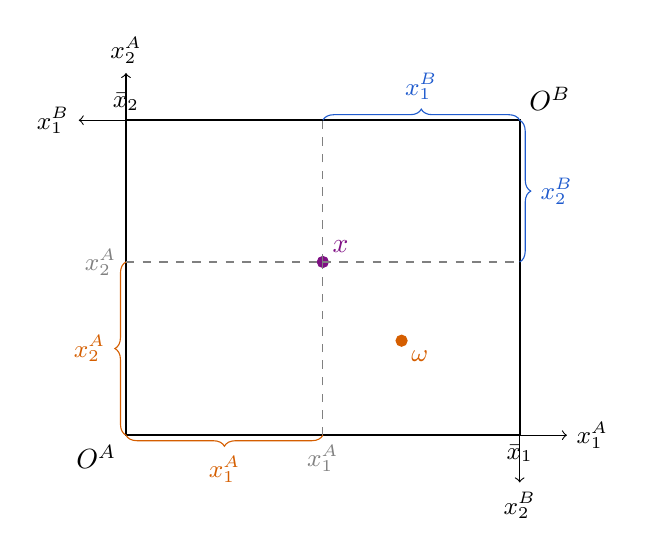
\begin{tikzpicture}[scale=1.0]
  %% Box
  \draw[thick] (0,0) rectangle (5,4);

  %% Axes for individual 1 (origin bottom-left)
  \draw[->] (0,0) -- (5.6,0) node[right] {\small $x_1^A$};
  \draw[->] (0,0) -- (0,4.6) node[above] {\small $x_2^A$};

  %% Axes for individual 2 (origin top-right, flipped)
  \draw[->] (5,4) -- (-0.6,4) node[left] {\small $x_1^B$};
  \draw[->] (5,4) -- (5,-0.6) node[below] {\small $x_2^B$};

  %% Origin labels
  \node[below left] at (0,0) {$O^A$};
  \node[above right] at (5,4) {$O^B$};

  %% Total endowment labels
  \node[below] at (5,0) {\small $\bar{x}_1$};
  \node[above]  at (0,4) {\small $\bar{x}_2$};

  %% A generic allocation point
  \filldraw[NTHU1] (2.5,2.2) circle (2pt) node[above right] {$x$};

  %% Dashed lines to axes
  \draw[dashed, gray] (2.5,0) node[below] {\small $x_1^A$} -- (2.5,2.2);
  \draw[dashed, gray] (0,2.2) node[left]  {\small $x_2^A$} -- (2.5,2.2);
  \draw[dashed, gray] (2.5,2.2) -- (2.5,4);
  \draw[dashed, gray] (2.5,2.2) -- (5,2.2);
  %% Endowment point (initial allocation)
  \filldraw[red] (3.5,1.2) circle (2pt) node[below right] {\small  $\omega$};

  %% Shaded feasible region (whole box)
  %% (box itself is the feasible set -- no shading needed)

  %% Dimension braces
  \draw[decorate, decoration={brace, mirror, amplitude=4pt}, red]
    (0,0) -- (2.5,0) node[midway, below=4pt] {\small $x_1^A$};
  \draw[decorate, decoration={brace, amplitude=4pt}, red]
    (0,0) -- (0,2.2) node[midway, left=4pt] {\small $x_2^A$};
  \draw[decorate, decoration={brace, amplitude=4pt}, blue]
    (2.5,4) -- (5,4) node[midway, above=4pt] {\small $x_1^B$};
  \draw[decorate, decoration={brace, mirror, amplitude=4pt}, blue]
    (5,2.2) -- (5,4) node[midway, right=4pt] {\small $x_2^B$};
\end{tikzpicture}
\end{column}
\begin{column}{0.42\textwidth}
Edgeworth box
\begin{itemize}\setlength\itemsep{5pt}
  \item Individual A,B and goods 1,2
  \item Total endowments:
  $\bar{x}_1$  and $\bar{x}_2$ 
  \item Every point inside the box is a feasible allocation 
  \item $O^i$: origin for $i\in\{A,B\}$
  
  \item Point $\omega$: initial endowment
  (pre-trade allocation)
  \item $x$ is one possible trade
  \item Is this desirable?
\end{itemize}
\end{column}
\end{columns}
\end{frame}


\begin{frame}
\frametitle{Pareto efficiency and contract curve} 
\begin{columns}
\begin{column}{0.55\textwidth}
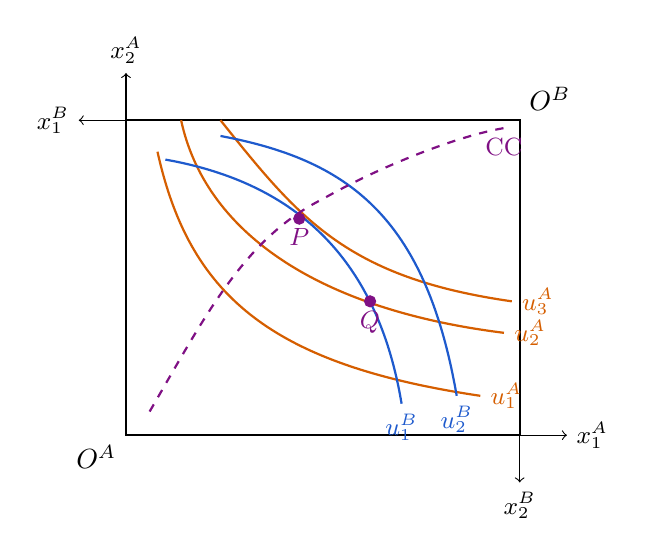
\begin{tikzpicture}[scale=1.0]
  %% Box
  \draw[thick] (0,0) rectangle (5,4);

  %% Axes A (origin bottom-left)
  \draw[->] (0,0) -- (5.6,0) node[right] {\small $x_1^A$};
  \draw[->] (0,0) -- (0,4.6) node[above] {\small $x_2^A$};

  %% Axes B (origin top-right)
  \draw[->] (5,4) -- (-0.6,4) node[left]  {\small $x_1^B$};
  \draw[->] (5,4) -- (5,-0.6) node[below] {\small $x_2^B$};

  %% Origin labels
  \node[below left]  at (0,0) {$O^A$};
  \node[above right] at (5,4) {$O^B$};

  %% Indifference curves for A
  %% Convex from O^A: open toward top-right
  \draw[thick, red]
    (0.4,3.6) .. controls (0.8,1.8) and (1.8,0.9) .. (4.5,0.5)
    node[right] {\small $u^A_1$};
  \draw[thick, red]
    (0.7,4.0) .. controls (1.0,2.6) and (2.4,1.6) .. (4.8,1.3)
    node[right] {\small $u^A_2$};
  \draw[thick, red]
    (1.2,4) .. controls (2.2,2.75) and (2.8,2) .. (4.9,1.7)
    node[right] {\small $u^A_3$};


  %% Indifference curves for B
  %% Convex from O^B: open toward bottom-left
  %% From O^A's perspective: concave, bulging toward bottom-left
  \draw[thick, blue]
    (0.5,3.5) .. controls (2.2,3.2) and (3.2,2.2) .. (3.5,0.4)
    node[below] {\small $u^B_1$};
  \draw[thick, blue]
    (1.2,3.8) .. controls (2.8,3.5) and (3.8,2.8) .. (4.2,0.5)
    node[below] {\small $u^B_2$};

  %% Endowment point
  %\filldraw[black] (2.8,1.6) circle (2pt) node[below right] {\small $\omega$};

  %% Tangency points
  \filldraw[NTHU1] (2.2,2.75) circle (2pt) node[below] {\small $P$};
  \filldraw[NTHU1] (3.1,1.7) circle (2pt) node[below] {\small $Q$};



  %% Contract curve: runs from O^A to O^B
  \draw[thick, NTHU1, dashed]
    (0.3,0.3) .. controls (1.0,1.5) and (1.5,2.5) ..
    (2.5,3.0) .. controls (3.2,3.4) and (4.2,3.8) .. (4.8,3.9)
    node[below] {\small CC};


\end{tikzpicture}
\end{column}
\begin{column}{0.42\textwidth}
Pareto efficient allocation
\begin{itemize}\setlength\itemsep{5pt}
  \item \textcolor{red}{$u_1^A, u_2^A$}:
  $A$'s indifference curves
  \item \textcolor{blue}{$u_1^B,u_2^B$}:
  $B$'s indifference curves
  \item $Q$: Current allocation
  \begin{itemize}\setlength\itemsep{5pt}
    \item $u_A$ rises with $x_1^A\downarrow$, $x_2^A\uparrow$ 
    \item $u_B$ rises with $x_2^A\uparrow$, $x_2^A\downarrow$ 
    \item $Q$ is thus not Pareto efficient
  \end{itemize}
  \item $P$: Pareto efficient
  \begin{itemize}\setlength\itemsep{5pt}
    \item Any departure: $u^A\downarrow$ or $u^B\downarrow$
    \item Tangent indifference curves
  \end{itemize}
  \item \textbf{CC}: contract curve ---
  locus of all Pareto efficient
  allocations
\end{itemize}
\end{column}
\end{columns}
\end{frame}


\begin{frame}
\frametitle{Pareto efficiency in mathematics}
Conditions for Pareto efficient allocation 
\begin{itemize}\setlength\itemsep{3pt}
\item Marginal rate of substitution between good 1 and 2 ($MRS_{1,2} = \frac{MU_1}{MU_2}=\frac{u_1'}{u_2'}$) 
\begin{itemize}\setlength\itemsep{3pt}
\item Rate at which consumer is willing to trade two goods while keeping utility same
\item Subjective value of good 1 in terms of good 2 that keeps utility same
\item It is the slope of the indifference curves
\end{itemize}
\item Pareto efficient allocation in exchange economy: $MRS_{1,2}^A=MRS_{1,2}^B$
\begin{itemize}\setlength\itemsep{3pt}
\item Indifference curves of both $A$ and $B$ are tangent to each other
\end{itemize}
\item Intuitively, suppose $MRS_{1,2}^A=1$ and $MRS_{1,2}^B=2$
\begin{itemize}\setlength\itemsep{3pt}
\item $A$ is willing to trade 1 unit of good 1 with 1 unit of good 2 
\item $B$ is willing to trade 1 unit of good 1 with 2 units of good 2 
\item Suppose $A$ gives up 1 unit of good 1 and gets 2 units of good 2
 \item $u^A \uparrow$ by an amount equal to one extra unit 
  of good 1, while $u^B$ stays the same
\item Thus, a pareto improvement is possible $\to$ pre-trade allocation is not pareto efficient
\end{itemize}
\end{itemize}
\end{frame}

\begin{frame}
\frametitle{Two welfare theorems}
\begin{block}{Two Welfare Theorems}
\begin{itemize}\setlength\itemsep{3pt}
\item First Welfare Theorem: A competitive equilibrium is Pareto efficient
\item Second Welfare Theorem: Any Pareto efficient allocation can be achieved as a competitive equilibrium, following an appropriate redistribution of endowments\\
\end{itemize}
\end{block} \medskip
Takeaways
\begin{itemize}\setlength\itemsep{3pt}
  \item Markets can achieve Pareto efficient allocation without intervention (1st thm)
  \begin{itemize}\setlength\itemsep{3pt}
  \item Competitive prices lead each consumer to set 
  $MRS^i_{12} = p_1/p_2$ for all $i$
  \end{itemize}
  \item However, Pareto efficient allocations may not be desirable in terms of equality
   \begin{itemize}
  \item \textit{Any} allocation on the contract curve is pareto efficient
  \end{itemize}

  \item Taxes can redistribute toward a socially preferred allocation (2nd)
  \item That comes with welfare costs (dedweight loss quantified earlier)
\end{itemize}
\end{frame}

\begin{frame}
\frametitle{Formalizing the redistribution questions}
Social Welfare Function
\begin{itemize}\setlength\itemsep{3pt}
  \item A function reflecting how utilities of its members affect the society as a whole
  \item Generic notation
  \[
  W = F(u^A, u^B)
  \]\vspace{-10pt}
  \item Different functional forms and tax instruments lead to different conclusions
  \begin{itemize}\setlength\itemsep{3pt}
  \item Utilitarian function: $u^A+ u^B$ - Simple sum of utilities
    \item Weighted sum of utilities: $\alpha u^A + (1-\alpha)u^B$ - Can put different weights on $A$ and $B$
    \item Rawlsian function: $\min{\{u^A, u^B\}}$ - Maximizing the welfare of the poorest
  \end{itemize}
  \item Government maximizes social welfare function subject to budget constraint, typically
  \[
  \max_{t_i} W \ \text{subject to (s.t.)} \ \sum_{i} t_i x_i \geq R
  \]
  i.e. its (tax) revenues  $\geq R$ (to be spent on public goods and redistribution)
\end{itemize}
\end{frame}

\section{Optimal Consumption Taxation}
\begin{transitionframe}
\begin{center}
  \begin{huge}
    \textcolor{NTHU1}{%
  Optimal Consumption Taxation
    }
  \end{huge}
\end{center}
\end{transitionframe}

% Two ways to view welfare loss
% one in terms of utilities: loss in utility not recovered by taxation
% One in terms of revenues: "Excess burden" of taxation, or welfare cost of raising one dollar of revenue above and beyond the dollar itself


% Then formu
\subsection{Consumer choice and deadweight loss}



\begin{frame}
\frametitle{Calculating deadweight loss with one good} 
\begin{columns}
\begin{column}{0.45\textwidth}
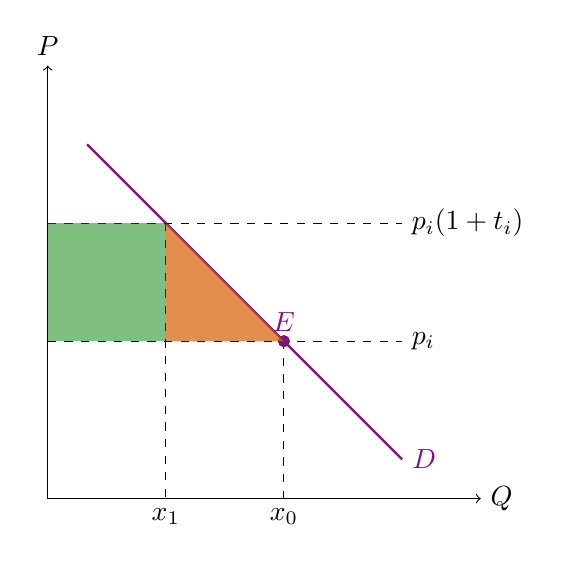
\begin{tikzpicture}[scale=1.0]
  %% 1. Axes
  \draw[->] (0,0) -- (5.5,0) node[right] {$Q$};
  \draw[->] (0,0) -- (0,5.5) node[above] {$P$};
  %% 2. Curves
  \draw[thick, color=NTHU1] (0.5,4.5) -- (4.5,0.5) node[right] {$D$};
  \draw[dashed, color=black]  (0,2) -- (4.5,2) node[right] {$p_i$};
  \draw[dashed, color=black]  (0,3.5) -- (4.5,3.5) node[right] {$p_i(1+t_i)$};

  \draw[dashed, color=black]  (1.5,3.5) -- (1.5,0) node[below] {$x_1$};
  \draw[dashed, color=black]  (3,2) -- (3,0) node[below] {$x_0$};
  %% 3. Points and labels

  
  \filldraw[NTHU1] (3,2) circle (2pt) node[above] {$E$};
  %% 4. Shaded regions
  \fill[red, opacity=0.7] (1.5,2) -- (1.5,3.5) -- (3,2) -- cycle;
  \fill[green, opacity=0.5] (0,2) -- (1.5,2) -- (1.5,3.5) -- (0,3.5) -- cycle;
\end{tikzpicture}
\end{column}
\begin{column}{0.55\textwidth}
Tax rate of $t_i$
\begin{itemize}\setlength\itemsep{3pt}
\item $\Delta X = X_1-X_0 (<0)$, and $\Delta P=pt_i (>0)$
\item Calculating the triangle: $-\frac{1}{2}\Delta X \Delta P$
\end{itemize}\medskip

More general expression of deadweight loss
\begin{itemize}\setlength\itemsep{3pt}
\item Demand elasticity: $\epsilon_d=-\frac{\Delta X/X}{\Delta P/P}=-  \frac{\Delta X}{\Delta P}\frac{P}{X} $
\item From this, we can write deadweight loss as
\[\footnotesize
DWL = \frac{1}{2} \underbrace{\left(\epsilon_d \Delta P \frac{X}{P}\right)}_{-\Delta X} \Delta P =\frac{1}{2}\epsilon_d P X t^2
\]\vspace{-10pt}
\item Larger DWL with higher tax and elasticity
\end{itemize}
\end{column}
\end{columns}
\end{frame}


\begin{frame}
\begin{columns}
  \begin{column}{0.45\textwidth}
\frametitle{Analyzing effects of price change with income and substition effects} 
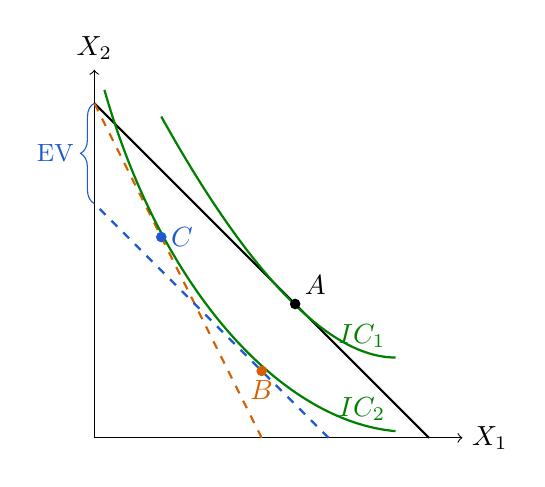
\begin{tikzpicture}[scale=0.85]
  \draw[->] (0,0) -- (5.5,0) node[right] {$X_1$};
  \draw[->] (0,0) -- (0,5.5) node[above] {$X_2$};
  %% Original budget line
  \draw[thick, black] (5,0) -- (0,5);
  %% Post-tax budget line
  \draw[thick, red, dashed] (2.5,0) -- (0,5);
  %% Compensated (Hicksian) budget line — same slope as post-tax, tangent to original IC
  \draw[thick, blue, dashed] (3.5,0) -- (0,3.5);
  %% Indifference curves (hand-drawn approximations as bezier)
\draw[thick, green] (1,4.8) .. controls (2,3) and (3.3,1.2) .. (4.5,1.2) node[above left] {$IC_1$};
  \draw[thick, green] (0.15,5.2) .. controls (1,2.2) and (2.8,0.25) .. (4.5,0.1) node[above left] {$IC_2$};
  %% Three points
  \filldraw[black] (3,2) circle (2pt) node[above right] {$A$};
  \filldraw[blue]  (1,3) circle (2pt) node[right] {$C$};
  \filldraw[red]   (2.5,1) circle (2pt) node[below] {$B$};
  \draw[decorate, decoration={brace,mirror, amplitude=5pt}, blue]
    (0,5) -- (0,3.5) node[midway, left=4pt] {\small EV};
\end{tikzpicture}
\end{column}
\begin{column}{0.55\textwidth}
Suppose price of $X_1$ rises twofold
\begin{itemize}
\item Budget constraint tilts inward
\item Consumption $A \to C$, Utility $IC_1 \to IC_2$
\end{itemize}\medskip
Question to quantify welfare changes
\begin{itemize}
\item What amount of change in income (based on old prices) lead to new IC?
\end{itemize}\medskip
Income and substitution effects
\begin{itemize}
\item Income: Changes in (real) income: $A\to B$
\item Substitution: Change in relative price: $B\to C$
\end{itemize}\medskip
Note: Change in income (before price change) leading to new IC is \textit{Equivalent variation} (EV)
\end{column}
\end{columns}
\end{frame}

\begin{frame}
\frametitle{Other way to analyze effect of price changes} 
\begin{columns}
  \begin{column}{0.45\textwidth}
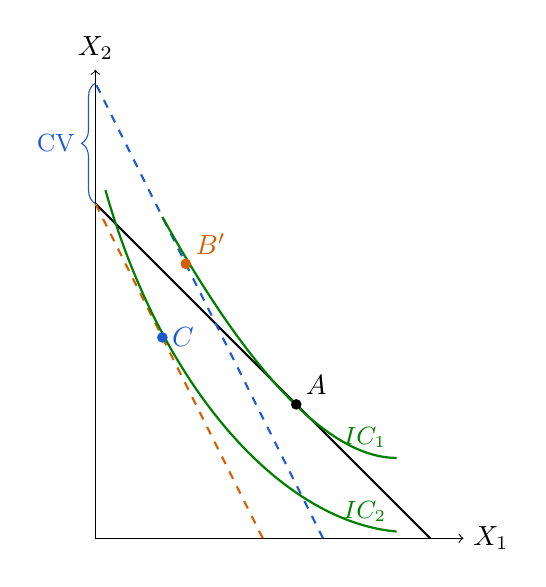
\begin{tikzpicture}[scale=0.85]
  \draw[->] (0,0) -- (5.5,0) node[right] {$X_1$};
  \draw[->] (0,0) -- (0,7) node[above] {$X_2$};
  %% Original budget line
  \draw[thick, black] (5,0) -- (0,5);
  %% Post-tax budget line
  \draw[thick, red, dashed] (2.5,0) -- (0,5);
  %% Compensated (Hicksian) budget line — same slope as post-tax, tangent to original IC
  \draw[thick, blue, dashed] (3.4,0) -- (0,6.8);
  %% Indifference curves (hand-drawn approximations as bezier)
  \draw[thick, green] (1,4.8) .. controls (2,3) and (3.3,1.2) .. (4.5,1.2)  node[above left] {\small $IC_1$};
  \draw[thick, green] (0.15,5.2) .. controls (1,2.2) and (2.8,0.25) .. (4.5,0.1)  node[above left] {\small $IC_2$};
  %% Three points
  \filldraw[black] (3,2) circle (2pt) node[above right] {$A$};
  \filldraw[blue]  (1,3) circle (2pt) node[right] {$C$};
  \filldraw[red]   (1.35,4.1) circle (2pt) node[above right] {$B'$};
  \draw[decorate, decoration={brace,mirror, amplitude=5pt}, blue]
    (0,6.8) -- (0,5) node[midway, left=4pt] {\small CV};
\end{tikzpicture}
\end{column}
\begin{column}{0.55\textwidth}
Same situation, but different question
\begin{itemize}
\item How much income compensation (based on new prices) are required to return to old IC?
\end{itemize}\medskip
Income and substitution effects
\begin{itemize}
\item Substitution: $x_2$ relatively cheaper:  $A\to B'$
\item Income: (Real) income falls: $B'\to C$
\end{itemize}\medskip
The income compensation required to preserve old IC is \textit{compensating variation} (CV)
\begin{itemize}
\item EV and CV usually differ ($\because$ different IC used)
\end{itemize}
\end{column}
\end{columns}
\end{frame}

\begin{frame}
\frametitle{Ad valorem tax vs lump sum tax}
Advalorem tax
\begin{itemize}\setlength\itemsep{3pt}
\item A tax that is proportional to the transaction, such that 
\[
P_{\text{post-tax}}=P(1+t)
\]
\item Budget constraint: $P_{1}X_1(1+t_1)+P_2X_2 = I$
\item Distortionary: Change relative price $\to$ Shift consumption to untaxed good
\item Substitution and income effect present
\end{itemize} \medskip


Lump-sum taxation
\begin{itemize}\setlength\itemsep{3pt}
\item A tax where no change in behavior can affect the amount (same tax no matter what)
\item Budget constraint: $P_{1}X_1+P_2X_2 = I-T$
\item No change in relative price, only income effect 
\end{itemize} \medskip
\end{frame}

\begin{frame}
\begin{columns}
  \begin{column}{0.45\textwidth}
\frametitle{Excess burden: Hypothetical lump-sum vs consumption tax} 
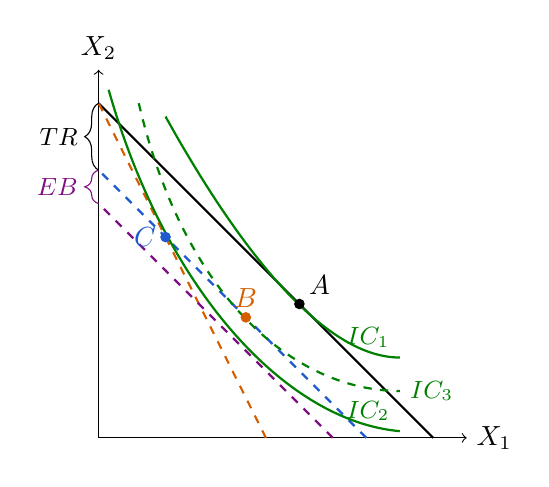
\begin{tikzpicture}[scale=0.85]
  \draw[->] (0,0) -- (5.5,0) node[right] {$X_1$};
  \draw[->] (0,0) -- (0,5.5) node[above] {$X_2$};
  %% Original budget line
  \draw[thick, black] (5,0) -- (0,5);
  %% Post-tax budget line
  \draw[thick, red, dashed] (2.5,0) -- (0,5);
  %% Compensated (Hicksian) budget line — same slope as post-tax, tangent to original IC
  \draw[thick, blue, dashed] (4,0) -- (0,4);
  \draw[thick, NTHU1, dashed] (3.5,0) -- (0,3.5);
  %% Indifference curves (hand-drawn approximations as bezier)
\draw[thick, green] (1,4.8) .. controls (2,3) and (3.3,1.2) .. (4.5,1.2) node[above left] {\small $IC_1$};
\draw[thick,dashed, green] (0.6,5) .. controls (1.3,2) and (3,0.7) .. (4.5,0.7) node[right] {\small $IC_3$};
  \draw[thick, green] (0.15,5.2) .. controls (1,2.2) and (2.8,0.25) .. (4.5,0.1) node[above left] {\small $IC_2$};
  %% Three point
  \filldraw[black] (3,2) circle (2pt) node[above right] {$A$};
  \filldraw[blue]  (1,3) circle (2pt) node[left] {$C$};
  \filldraw[red]   (2.2,1.8) circle (2pt) node[above] {$B$};
  \draw[decorate, decoration={brace,mirror, amplitude=5pt}, NTHU1]
    (0,4) -- (0,3.5) node[midway, left=4pt] {\small $EB$};
    \draw[decorate, decoration={brace,mirror, amplitude=5pt}, black]
    (0,5) -- (0,4) node[midway, left=4pt] {\small $TR$};
\end{tikzpicture}
\end{column}
\begin{column}{0.55\textwidth}
Ad valorem and lump-sum with equal TR
\begin{itemize}
\item Lump-sum tax: $A\to B$, and $IC_1 \to IC_3$
\item Ad valorem tax: $A\to C$, and $IC_1 \to IC_2$ 
\item Assuming both are normal goods, $IC_2 < IC_3$
\item $EB$: The difference in the utility 
\item This captures additional utility from distortionary taxes
\end{itemize}
\end{column}
\end{columns}
\end{frame}



\begin{frame}
\begin{columns}
  \begin{column}{0.45\textwidth}
\frametitle{Excess burden: Loss in utilty not made up for in taxes} 
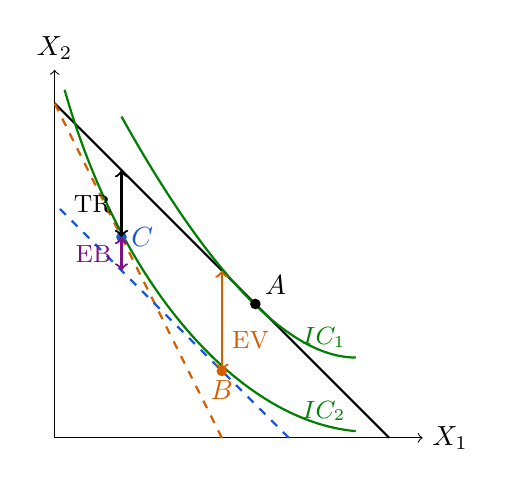
\begin{tikzpicture}[scale=0.85]
  \draw[->] (0,0) -- (5.5,0) node[right] {$X_1$};
  \draw[->] (0,0) -- (0,5.5) node[above] {$X_2$};
  %% Original budget line
  \draw[thick, black] (5,0) -- (0,5);
  %% Post-tax budget line
  \draw[thick, red, dashed] (2.5,0) -- (0,5);
  %% Compensated (Hicksian) budget line — same slope as post-tax, tangent to original IC
  \draw[thick, blue, dashed] (3.5,0) -- (0,3.5);
  %% Indifference curves (hand-drawn approximations as bezier)
\draw[thick, green] (1,4.8) .. controls (2,3) and (3.3,1.2) .. (4.5,1.2) node[above left] {\small $IC_1$};
  \draw[thick, green] (0.15,5.2) .. controls (1,2.2) and (2.8,0.25) .. (4.5,0.1) node[above left] {\small $IC_2$};
  %% Three points
  \filldraw[black] (3,2) circle (2pt) node[above right] {$A$};
  \filldraw[blue]  (1,3) circle (2pt) node[right] {$C$};
  \filldraw[red]   (2.5,1) circle (2pt) node[below] {$B$};
  %% Braces
  \draw[<->, thick, black] (1,3) -- (1,4)  node[midway,left] {\small TR};
  \draw[<->, thick, NTHU1] (1,2.5) -- (1,3) node[midway,left] {\small EB};
  \draw[<->, thick, red]   (2.5,1) -- (2.5,2.5) node[midway,below right] {\small EV};
\end{tikzpicture}
\end{column}
\begin{column}{0.55\textwidth}
Consumption tax on $X_1$ ($X_2$ not taxed)
\begin{itemize}
\item Consume $A\to C$, Utility $IC_1 \to IC_2$
\item $EV$: Welfare loss from tax
\item $TR$: Tax revenue in terms of $X_2$ per unit of $X_1$
\item $EB$ is not made up for by anyone
\item Thus, $EB$ captures efficiency cost from distortionary taxation
\end{itemize}\medskip
\end{column}
\end{columns}
\end{frame}

\begin{frame}
\frametitle{Taxation in practice} 
Lump-sum tax must be independent of all observable behavior
\begin{itemize}\setlength\itemsep{3pt}
\item In reality, this is not the case
\item Observable proxies -- income, consumption etc -- are subject to behavioral response
\begin{itemize}\setlength\itemsep{3pt}
\item People underreport income/wealth, shift compensation to non-taxable forms
\end{itemize}
\item Ideal lump-sum tax is based on innate ability, which is \textit{private information}
\begin{itemize}\setlength\itemsep{3pt}
\item No way to objectively verify: Some individuals can pretend to be of different type
\end{itemize}
\item Thus, \textit{all} taxes are distortionary $\to$ Optimal tax to minimize efficiency cost
\end{itemize}\medskip
Why tax at all if distortions exist?
\begin{itemize}\setlength\itemsep{3pt}
\item Distortions are measured relative to a perfectly competitive market
\item In reality, markets failures exist $\to$ Taxation may improve welfare
\begin{itemize}\setlength\itemsep{3pt}
\item Externalities, monopolies, public goods, information asymmetry
\item In developing countries, markets may not even exist $\to$ Government as sole provider
\end{itemize}
\end{itemize}
\end{frame}

\subsection{Ramsey taxation rules}
\begin{frame}
\frametitle{Optimal taxation with multiple goods: Inverse elasticity rule}
Setup 
\begin{itemize}\setlength\itemsep{3pt}
\item Assume two goods -- $X_1$ and $X_2$ -- are being taxed
\begin{itemize}
\item Both goods are independent of each other (neither complement nor substitute)
\end{itemize}
\item Optimal taxes minimize deadweight loss while obtaining tax revenue $R$
\[
\begin{aligned}
\text{Objective:  } &\min_{t_1, t_2} \frac{1}{2}\left[P_1X_1\epsilon_1t_1^2+P_2X_2\epsilon_2 t_2^2\right]\\
\text{Constraint:  }& t_1P_1X_1+t_2P_2X_2 \geq R
\end{aligned}
\]
\item Solve :$\mathcal{L}=\frac{1}{2}\left[P_1X_1\epsilon_1t_1^2+P_2X_2\epsilon_2 t_2^2\right] + \lambda[t_1P_1X_1+t_2P_2X_2 - R]$
\begin{itemize}\setlength\itemsep{3pt} 
  \item F.O.C.[$t_i$]: $P_iX_i\epsilon_it_i+P_iX_i\lambda=0$ for $i\in\{1,2\}$

\end{itemize}
\item The inverse elasticity rule
\[
\frac{t_1}{t_2} = \frac{\epsilon_2}{\epsilon_1}=\frac{1/\epsilon_1}{1/\epsilon_2}
\]

\end{itemize}
\end{frame}

\begin{frame}
\frametitle{Optimal taxation with multiple goods: Inverse elasticity rule}
Implications of the inverse elasticity rule
\begin{itemize}\setlength\itemsep{3pt}
\item Using $\epsilon_i = -\frac{\Delta X_i}{X_i}\frac{P_i}{\Delta P_i}$ and $\Delta P_i = P_it_i$, we can write
\[
\frac{t_1}{t_2} = \frac{\epsilon_2}{\epsilon_1}\iff\frac{t_1}{t_2} = \frac{-\frac{\Delta X_2}{X_2}\frac{1}{t_2}}{-\frac{\Delta X_1}{X_1}\frac{1}{t_1}}\iff \frac{\Delta X_1}{X_1}=\frac{\Delta X_2}{X_2}
\]
\item Tax rate should be higher for goods for those with lower elasticity
\item Tax rate should be set to equalize percent change in quantities demanded
\end{itemize}\medskip
Equity implications
\begin{itemize}
\item Necessities tend to have lower elasticity, luxuries higher
\item Could result in tax burden going to low-income persons
\end{itemize}
\end{frame}

\begin{frame}
\frametitle{Generalized version: Ramsey taxation rule (Ramsey (1927))}
Setup
\begin{itemize}\setlength\itemsep{3pt}
\item Now we assume that demand for $X_1$ and $X_2$ can be interdependent
\begin{itemize}\setlength\itemsep{3pt}
\item i.e. Tax of $X_1$ affects demand for $X_1$ and $X_2$
\end{itemize}
Define Cross-elasticity of good 1 and 2 as
\[
\epsilon_{1,2}= \frac{\partial X_1/X_1}{\partial P_2/P_2}=\frac{\partial X_1}{X_1}\frac{P_2}{\partial P_2}
\]
\item Change in demand for good 1, $X_1(P_1,P_2)$  can be broken into (total differentiation)
 \[
 \Delta X_1 = \frac{\partial X_1}{\partial P_1}\Delta P_1+\frac{\partial X_1}{\partial P_2}\Delta P_2 \iff \epsilon_{1,1} \frac{X_1}{P_1}\Delta P_1+\epsilon_{1,2} \frac{X_1}{P_2}\Delta P_2 
\]
\item Across two goods, total deadweight loss is now
\[
DWL = \frac{1}{2}\sum_{i=1}^2\sum_{j=1}^2 \left[\left(\epsilon_{i,j}\frac{X_i}{P_j}\Delta P_j\right) \Delta P_i\right]=\frac{1}{2}\sum_{i=1}^2\sum_{j=1}^2 \epsilon_{i.j}P_iX_it_it_j
\]
\end{itemize}
\end{frame}


\begin{frame}
\frametitle{Generalized version: Ramsey taxation rule (Ramsey (1927))}
Solving for the optimal tax
\begin{itemize}\setlength\itemsep{3pt}
\item Lagrangian takes the following form
\[
\mathcal{L}=\frac{1}{2}\sum_{i=1}^2\sum_{j=1}^2 \epsilon_{i.j}P_iX_it_it_j + \mu[t_1P_1X_1+t_2P_2X_2 - R]
\]
\item First order conditions on tax rates
\[
[t_i]: \frac{1}{2}[2\epsilon_{i,i}P_iX_it_i+\epsilon_{i,j}P_iX_it_j+\epsilon_{j,i}P_jX_jt_j]+\mu P_iX_i=0
\]
\item We rely on Slutsky symmetry: Cross-price substitution effect of good i on good j = Cross-price substitution effect of good j on good i
\[
\frac{\partial X_i}{\partial P_j}=\frac{\partial X_j}{\partial P_i} \iff \epsilon_{i,j}\frac{X_i}{P_j}=\epsilon_{j,i}\frac{X_j}{P_i} \iff\epsilon_{i,j}X_i P_i=\epsilon_{j,i} X_j P_j
\]
\end{itemize}
\end{frame}


\begin{frame}
\frametitle{Generalized version: Ramsey taxation rule (Ramsey (1927))}
Solving for the optimal tax
\begin{itemize}\setlength\itemsep{3pt}
\item The first order conditions become
\[
\epsilon_{i,i}P_iX_it_i + \epsilon_{i,j}P_iX_it_j = -\mu P_iX_i \iff \sum_{j=1}^2 \epsilon_{i,j}t_j=-\mu
\]
\end{itemize}
Intuition
\begin{itemize}
  \item Elasticity weighted sum of tax rates should equal a constant
  \item That means elastic goods are taxed low, inelastic goods high
  \item Low-income personss relying heavily on necessities worse off?
  \item Solve with many-person framework: Higher welfare weights to low-income persons
\end{itemize}
\end{frame}




\section{Optimal Income Taxation}
\subsection{Linear taxation}
\begin{transitionframe}
\begin{center}
  \begin{huge}
    \textcolor{NTHU1}{%
  Optimal Income Taxation
    }
  \end{huge}
\end{center}
\end{transitionframe}


\begin{frame}
\frametitle{Design of optimal income tax: How to balance equity and efficiency}

Equity motivation
\begin{itemize}\setlength\itemsep{3pt}
    \item Individuals differ in earning capacity $w$ --- ability, family background, human capital
    \item These differences are largely outside individual control
    \item If $u''(c) < 0$, transferring \$1 from rich to poor raises total welfare
    \[
        u'(c_L) > u'(c_H) \iff \text{marginal utility higher for the poor}
    \]
\item Redistribution raises social welfare --- but trade-off with efficiency cost exists
\end{itemize}\medskip
The fundamental tension: Balancing efficiency and equity
\begin{itemize}\setlength\itemsep{3pt}
    \item We want to tax according to ability $w$ (vertical equity) 
    \item But $w$ is \textit{unobservable}, only income $z = wl$ is observable
    \item Taxing $z$ penalizes effort alongside ability --- efficiency cost of redistribution
    \item Yet failing to redistribute leaves inequality from factors outside individual control
\end{itemize}
\end{frame}

\begin{frame}
\frametitle{Equity consideration in taxes: Edgeworth Model}
Individuals utilities
\begin{itemize}\setlength\itemsep{3pt}
\item Individuals have same utility function $u(\cdot)$ that differs only in income
\item Pre-tax income $z_i$ is exogenously given, with tax being $T_i$ (lump-sum)
\item All remaining income is consumed: $c_i=z_i-T_i$
\end{itemize} \medskip
Government's decision on taxes
\begin{itemize}\setlength\itemsep{3pt}
\item Government maximizes sum of individual utilities
\item Subject to government budget constraint: Tax revenue at least greater than $R$
\item Lagrangian setup is as follows
\[
\mathcal{L}=\max_{T_i}\sum_{i=1}^n u(c_i)+\lambda\left[\sum_{i=1}^n T_i-R\right] \ \ \text{where} c_i = z_i-T_i
\]\vspace{-10pt}
\begin{itemize}
\item Replace $c_i$ with $Z_i-T_i$ and FOC w.r.t. $T_i$
\[
-u'(z_i-T_i)+\lambda=0 \iff u'(c_i)=\lambda \ \text{for all } i
\]
\end{itemize}
\end{itemize} \medskip
\end{frame}

\begin{frame}
\frametitle{Equity consideration in taxes: Edgeworth Model}
Takeaways from the conclusion
\[
 u'(c_i)=\lambda \ \text{for all } i
 \]\vspace{-10pt}
\begin{itemize}\setlength\itemsep{3pt}
\item Equal marginal utility of consumption for all
\item Since all have same preferences, taxes should be levied to equalize consumption
\item This can be seen as full insurance
\item As consumption is equalized, no incentive to work 
\end{itemize} \medskip
What modern optimal taxation achieves
\begin{itemize}\setlength\itemsep{3pt}
\item Balance between efficiency (minimize lost utilities) and equity (fairness)
\item Equity measured in terms of consumption inequality
\item Efficiency in terms of labor supply or productivity
\end{itemize} \medskip
\end{frame}

\begin{frame}
\frametitle{Linear income tax with labor supply decisions: Household decisions}

\begin{itemize}\setlength\itemsep{3pt}
\item Representative individual with wage $w$ chooses labor supply $l$ to maximize
$u(c, l)$ with $u_c =\frac{\partial u}{\partial c}> 0$, $u_l=\frac{\partial u}{\partial l} < 0$, facing:
\[
        c = (1-t)wl + a, \quad z = wl
\]
where $t$ is the flat tax rate and $a$ is the lump-sum transfer (or tax if $a<0$)
\item FOCs for Lagrangian $\mathcal{L}=u(c,l)+\lambda[(1-t)wl+a-c]$:
\[
    \begin{aligned}
\text{w.r.t }[c]:& \quad u_c -\lambda=0 \\
\text{w.r.t }[l]:& \quad u_l + \lambda(1-t)w=0\\
\Rightarrow &\quad-\frac{u_l}{u_c}=(1-t)w
    \end{aligned}
\]
\item Marginal disutility of labor in consumption units = marginal gain from work
\begin{itemize}\setlength\itemsep{3pt}
\item $t\uparrow$ $\to(1-t)w\downarrow \to -\frac{u_l}{u_c}>(1-t)w\to$ $l\downarrow$ to restore equality $\to$ $z\downarrow$
\end{itemize}
\end{itemize}
\end{frame}


\begin{frame}
\frametitle{Linear income tax with labor supply decisions: Government problem}
\begin{itemize}\setlength\itemsep{3pt}
\item Earnings $z(1-t) = wl$ respond to net-of-tax rate $(1-t)$ via labor supply decision. 
\item Government seeks to maximize revenue $R=t\cdot z(1-t)$

\item Define earnings elasticity with respect to net-of-tax rate:
\[
e = \frac{\partial z}{\partial(1-t)}\frac{(1-t)}{z} > 0
\]
\item Differentiating w.r.t $t$, we get: 
\[
\frac{dR}{dt} = z + t\frac{\partial z}{\partial t} =z - t\frac{\partial z}{\partial (1-t)} = z\left(1 - \frac{t}{1-t}e\right)
\]
\item Setting $\frac{dR}{dt} = 0$ gives the revenue-maximizing rate: $t=\frac{1}{1+e}$
\begin{itemize}\setlength\itemsep{3pt}
\item Any higher tax rates$\to$ Revenue falls $\to$ This is the laffer curve argument
\item Requires large $e$, but this argument is not realized as $e$ is known to be low (0.1 to 0.5)
\end{itemize}
\end{itemize}
\end{frame}

\begin{frame}
\frametitle{Linear income taxation: Optimal tax rate}
 With two types, raising $t$ by $dt$ has two effects:
\begin{itemize}\setlength\itemsep{3pt}
  \item Let $W(c_H, c_L)$ be the social welfare function
    \item \textit{Equity gain}: transfers resources from $H$ to $L$, raising social welfare if $W_{c_L}>W_{c_H}$
    \item \textit{Efficiency cost}: both types work less, shrinking the tax base by $e$
\end{itemize}\medskip
Optimal $t$ equates these two forces:
\[
\underbrace{\frac{t}{1-t}\cdot e}_{\text{efficiency cost}} = \underbrace{\frac{W_{c_L}-W_{c_H}}{W_{c_H}}}_{\text{equity gain}}
\]
\begin{itemize}
\item Higher $e$ $\Rightarrow$ lower $t^*$; stronger redistributive preference $\Rightarrow$ higher $t^*$
\item Any chance to tax high and low types differently? $\to$ Nonlinear taxation 
\end{itemize}
\end{frame}

\subsection{Nonlinear taxation}
\begin{frame}
\frametitle{Nonlinear income taxation: Setup}
Why not assign person-specific taxes $T_H \neq T_L$?
\begin{itemize}\setlength\itemsep{3pt}
  \item There are $a$ share of type $H$ (and $1-a$ of $L$)
    \item Government observes income $z = wl$ but \textit{not} ability $w$ directly
    \item Type $H$ can mimic type $L$ by working less (but keep ability): $l_H^{'} = \frac{z_L}{w_H} < l_L$
    \item Since $w_H > w_L$, mimicking costs $H$ less effort --- taxes for $L$ types may unravel
\end{itemize}\medskip
 Constraints of the government
\begin{itemize}
\item \textbf{Incentive compatibility (IC):}
\[
u\!\left(c_H, \frac{z_H}{w_H}\right) \geq u\!\left(c_L, \frac{z_L}{w_H}\right) \qquad
u\!\left(c_L, \frac{z_L}{w_L}\right) \geq u\!\left(c_H, \frac{z_H}{w_L}\right)
\]
\item \textbf{Budget constraint:}
\[
a\times\underbrace{(z_H - c_H)}_{\text{Tax on $H=T(z_H)$}} + (1-a)\times\underbrace{(z_L - c_L)}_{\text{Tax on $L=T(z_L)$}} \geq E
\]
\end{itemize}
\end{frame}

\begin{frame}
\frametitle{Nonlinear income taxation: Which IC binds?}
Not all ICs matter
\begin{itemize}\setlength\itemsep{3pt}
\item Two IC constraints --- but only one binds at the optimum
\item \textbf{Downward IC} ($H$ mimicking $L$) is the binding one:
\begin{itemize}\setlength\itemsep{3pt}
    \item $H$ finds mimicking $L$ relatively cheap --- high wage means less effort to earn $z_L$
    \item $L$ mimicking $H$ is prohibitively costly --- low wage requires enormous effort to earn $z_H$
\end{itemize}
\item So $L$'s IC is slack at the optimum --- set it aside and focus on $H$'s IC binding:
\[
u\!\left(c_H, \frac{z_H}{w_H}\right) = u\!\left(c_L, \frac{z_L}{w_H}\right)
\]
\end{itemize}
$H$ must be just indifferent between own bundle and $L$'s bundle (with its own ability)
\begin{itemize}\setlength\itemsep{3pt}
    \item Any more redistribution to $L$ would cause $H$ to mimic $L$ --- IC violated
    \item Better utility for $H$ with higher $C_H$? 
    \begin{itemize}
    \item Reduce $C_H$ and increase $C_L$ by slight amounts $\to$ Social welfare $\uparrow$ ($\because u'(c_H)<u'(c_L)$)
    \end{itemize}
    
    \item The binding IC is the key constraint limiting redistribution
\end{itemize}
\end{frame}

\begin{frame}
\frametitle{Nonlinear income taxation: Key results (Mirrlees, 1971)}
\textbf{No distortion at the top:} $T'(z_H) = 0$
\begin{itemize}\setlength\itemsep{3pt}
\item If $T'(z_H) > 0$, reducing it raises $H$'s labor supply 
\item It does not affect $L$'s labor or consumption $\to$ Pareto Improvement
\item Intuition: no one above $H$ to redistribute to --- distorting $H$ is pure efficiency loss
\end{itemize}\medskip
\textbf{Positive distortion at the bottom:} $T'(z_L) > 0$
\begin{itemize}\setlength\itemsep{3pt}
\item Distorting $L$ downward makes mimicking less attractive for $H$
\item Positive marginal rate for $L$ is the necessary cost of redistribution under hidden ability
\end{itemize}\medskip
Caveats in practice
\begin{itemize}\setlength\itemsep{3pt}
\item Ability is not fixed (human capital investments)
\item Top of the distribution is unknown, thus hard to know where to apply zero rate
\item Even richer models with dynamic taxation and endogenous skill formation
\end{itemize}
\end{frame}

\section{Conclusion}
\begin{transitionframe}
\begin{center}
  \begin{huge}
    \textcolor{NTHU1}{%
  Conclusion: Takeaways and open questions
    }
  \end{huge}
\end{center}
\end{transitionframe}

\begin{frame}{The Unified Logic of Optimal Taxation}
All three frameworks solve the same problem:\\
\medskip
\begin{itemize}\setlength\itemsep{3pt}
\item Raise revenue  
\item Achieving redistribution 
\item Minimize efficiency costs
\end{itemize}\medskip
They differ in \textit{what the government can observe}
\begin{center}
\begin{tabular}{lll}
  
\hline\hline
\textbf{Framework} & \textbf{Government observes} & \textbf{Key result} \\
\hline
Consumptionn tax & Goods, not utility & Inverse elasticity rule \\
Income tax & Income, not ability & Zero top marginal tax \\

\hline\hline
\end{tabular}
\end{center}
\bigskip
 As the government learns more about the taxpayer, the optimal tax system becomes more personalized --- and more efficient
\end{frame}

\begin{frame}{What the Theory Cannot Resolve}
Open tensions worth keeping in mind:
\begin{itemize}\setlength\itemsep{6pt}
    
    \item \textbf{The zero top rate:} clean in theory, but requires \textit{knowing where the distribution ends.} 
    \item \textbf{Correct social welfare function?:} Results are sensitive to the social welfare function. 
    \item \textbf{Dynamic taxation:} Types may change in reality (human capital accumulatio). Taxing high earners today may discourage skill acquisition
    \item \textbf{Informality:} In developing economies,  a large share of workers are outside the tax net entirely -- different theory required
   \item \textbf{Political economy:} Politicians may favor visible tax cuts over socially optimal design
   

\end{itemize}

\bigskip
\small\textit{Theory and practice diverge in many settings --- especially in developing countries. Is the gap a failure of policymakers to learn from theory, or of theory to reflect the constraints policymakers actually face?}
\end{frame}
%%%%%%%%%%%
\end{document}
